% !TEX root = WWW.tex
\section{Experimental Study}

We now  perform an experimental evaluation of our labeling scheme on a number of power-law networks.
The source code for our experiments can be found at:\\ \url{www.diku.dk/~simonsen/suppmat/www16/powerlaw.zip}

\subsection{Experimental Framework}\label{Sec:Experimental}
Recall that our labeling scheme separates  the nodes according to a selected threshold from the range $0 \dots \Delta$,\footnote{Recall that $\Delta$ is the graph's maximum degree.} which we select as a function of  the power-law parameter $\alpha$.
The following observation is the key to assess our labeling scheme's quality.
Suppose we chose a threshold  $n_0$ for a graph $G$, and call  the maximum label size of a thin node, $T(n_0)$ and the maximum label size of a fat node $F(n_0)$.  The size of our labeling scheme for the graph $G$ is the larger of these two values.
The critical observation is that, as our selection of threshold $n_0$ increases, $T(n_0)$ monotonically increases and  $F(n_0)$ monotonically decreases.
Our strategy thus arrives to optimality if we choose $n_0$ that minimises  the value $F(n_0)-T(n_0)$, in other words, where the curves of both functions intersect.
In the remainder of this section we call such threshold the \emph{empirical} threshold.

In contrast, we set the threshold in our labeling scheme as $\lceil \sqrt[\alpha]{C n/(\alpha-1)} \rceil$, which we denote as the \emph{predicted} threshold.
It is an approximation to the theoretically optimal threshold choice when degree distributions follow the power-law curve $k\mapsto Cn/k^\alpha$ perfectly, using integration as used in Proposition~\ref{prop:Contained}.

Note that a slow encoder can always arrive at the empirical threshold by a binary search which would incur an $O(\log n)$ factor on its running time. 
\paragraph{Performance Indicators}
We use the following to determine the quality of our labeling scheme:

\emph{Performance Indicator i:} We  compare the label sizes attained by our labeling schemes to other labeling schemes, namely state-of-the art labeling schemes for the classes of bounded-degree, sparse and general graphs using the  labeling schemes suggested in \cite{adjiashvili2014labeling},  Theorem~\ref{sparse-label} and \cite{alstrup2014adjacency}.  We interpret small label sizes for our scheme, especially in comparison with ``small'' classes like the class of bounded-degree graphs, as a sign that our labeling scheme efficiently utilizing  the extra information about the graphs: namely that their degree distribution is reasonably well-approximated by a power-law.

\emph{Performance Indicator ii:} We measure the difference in label sizes using the predicted and empirical thresholds. 
 We also measure  the difference between the predicted and empirical threshold in percentages with respect to the maximum degree.
We interpret a small relative differences in those as an evidence  that the predicted threshold can achieve small label sizes without examining the global properties of the network other than the power-law parameter $\alpha$. 
This best captures how close our ''guess" of the right threshold was, and will, in practice, allow for a faster encoding time.
 




 
 %\footnote{Additional notes on these values are found in Appendix~\ref{Section:TotalStorage}.

\paragraph{Test Sets}
We employ both real-world and synthetic data sets. 

The six \emph{synthetic} data sets are created by first generating a power-law degree sequence using the method of Clauset et al.~\cite[App.\ D]{clauset2009power}, subsequently constructing a corresponding graph for the sequence using the Havel-Hakimi method~\cite{hakimi1962realizability}. 
We use the range $2< \alpha < 3$ as suggested in~\cite{clauset2009power} as this range of $\alpha$ occurs most commonly in modeling of real-world networks. We generate graphs of $300,000$ and $1M.$ vertices denoted  s300$^{\alpha=x}$  and s1M$^{\alpha=x}$  respectively, for $x \in \{2.2,2.4,2.6,2.8\}$. 


The seven \emph{real-world} data sets originate  from articles that found the data to be well-approximated by a power-law. 
The \textsc{www} data set  \cite{albert1999internet} contains information on links between webpages within the nd.edu domain. 
The \textsc{enron} data set ~\cite{leskovec2009community}  contains email communication between  Enron employees (vertices are email addresses; there is a link between two addresses
if a mail has been sent between them).
The \textsc{internet} data set~\cite{newman} provides a snapshot the Internet structure at the level of  autonomous systems, reconstructed from BGP tables. 
For all of these sets, we consider the underlying simple, undirected graphs. For each set, standard maximum likelihood methods were used to compute the parameter
$\alpha$ of the best-fitting power-law curve \cite{clauset2009power}. Additional information on the data sets can be found in Table~\ref{t:datasets}.

\begin{table}[!ht]
\centering
\small
\begin{tabular}{lccccl}\hline
\multicolumn{6}{c}{Real-Life Graphs}\\\hline
Data set  & $\vert V \vert$ & $\vert E\vert$ & $\alpha$  & $\Delta_{\max}$ & Source\\\hline
\textsc{internet} &  22,963        &    48,436      & 2.09     & 2,390        & \cite{newman}\\
\textsc{enron}    &  36,692        &   183,830      & 1.97    &1,383         & \cite{leskovec2009community}\\
\textsc{www}      & 325,729        & 1,117,563     & 2.16 & 10,721            & \cite{albert1999internet}\\
\textsc{google} & 875,713 & 5,105,039 & 2.73 & 6,332 & \cite{leskovec2009community}\\
\textsc{Youtube} & 1,134,890 & 2,987,624 & 2.14 & 28,754 & \cite{yang2015defining}\\
\textsc{wikitalk} & 2,394,385 & 5,021,410 & 2.42 & 100,032 & \cite{leskovec2010predicting}\\
\textsc{LiveJournal} &  3,997,962        &    34,681,198      & 2.97     & 14,815        & \cite{yang2015defining}\\\hline


\multicolumn{6}{c}{Synthetic Graphs}\\\hline
s300$^{\alpha=2.2}$    & 300,000        & 491,926        & 2.2    & 10,906 & --\\
s300$^{\alpha=2.4}$    & 300,000        & 327,631        & 2.4    & 3,265 & --\\
s300$^{\alpha=2.6}$    & 300,000        & 261,949        & 2.6    & 1,410 & --\\
s300$^{\alpha=2.8}$    & 300,000        & 227,247        & 2.8    & 1,842 & --\\
s1M$^{\alpha=2.4}$    & 1,000,000       & 1,127,797      & 2.4    & 42,683 &-- \\
s1M$^{\alpha=2.6}$    & 1,000,000       & 878,472        & 2.6    & 12,169 &-- \\
s1M$^{\alpha=2.8}$    & 1,000,000       & 751,784         & 2.8   & 1,692  &-- \\\hline
\end{tabular}
\caption{Data sets and their properties. All graphs are undirected and simple. $\Delta_{\max}$ is the maximum degree of any vertex in the data set.}
\label{t:datasets}
\end{table}


\subsection{Findings}
Figure \ref{fig:findings} shows the distribution of maximum label sizes for two representative synthetic and  data sets. The maximum label size
for the predicted and empirical thresholds as well as upper bounds on the label sizes from different label schemes in the literature can be seen in Table \ref{t:labelsizes}. 
%Plots for the remaining data sets can be found in Appendix~\ref{App:ExpRes}.

\begin{figure*}[!ht]
\centering
\subfloat[\small s300$^{\alpha=2.2}$]{
    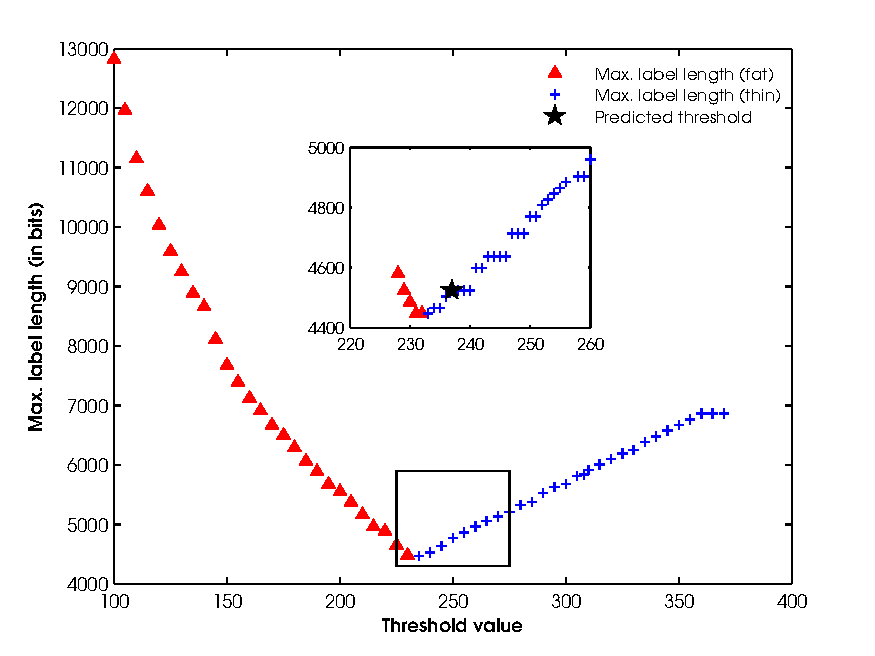
\includegraphics[width=0.4\textwidth]{Figures/synthetic-300k-alpha22.pdf}
    \label{f:fsyn300k}
}\hspace*{-2.5em}
\subfloat[\small \textsc{\small s1M$^{\alpha=2.2}$}]{
    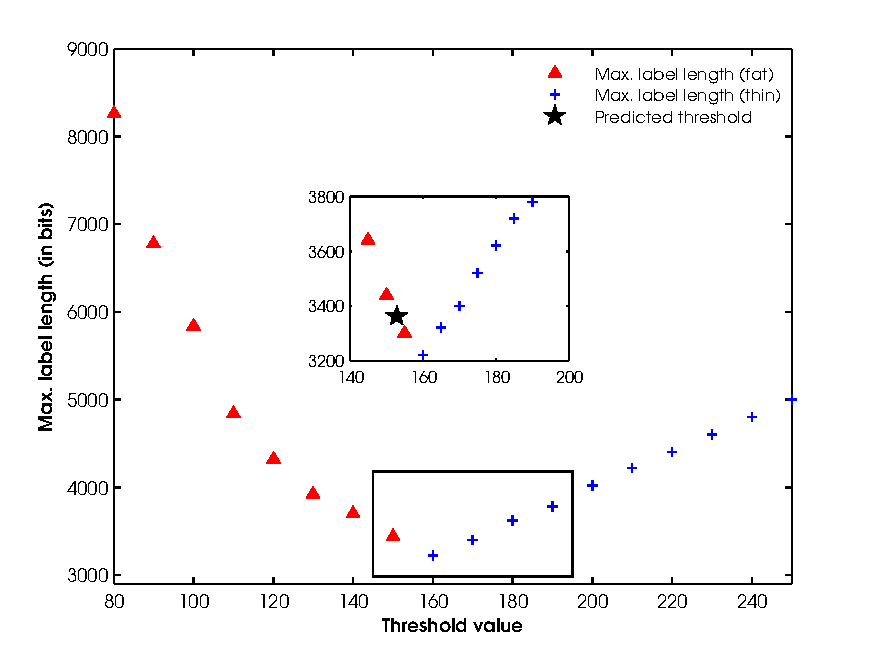
\includegraphics[width=0.4\textwidth]{Figures/synthetic-1M-26}
    \label{f:fsyn1M}
}%
\caption{Exemplary maximum label sizes of different threshold values for the synthetic data sets   s300$^{\alpha=2.2}$ and s1M$^{\alpha=2.6}$. 
The triangles and crosses represent that for the tested threshold the largest label belong to fat, resp. thin node. The star indicate the position of the predicted threshold.
See~\cite{} for the remaining  figures for synthetic datasets.}
\label{fig:findings}%
\end{figure*}

% !TEX root = WWW.tex
\begin{figure*}[!ht]
\centering
\subfloat[\small Fat and thin vertices vs. threshold values]{
    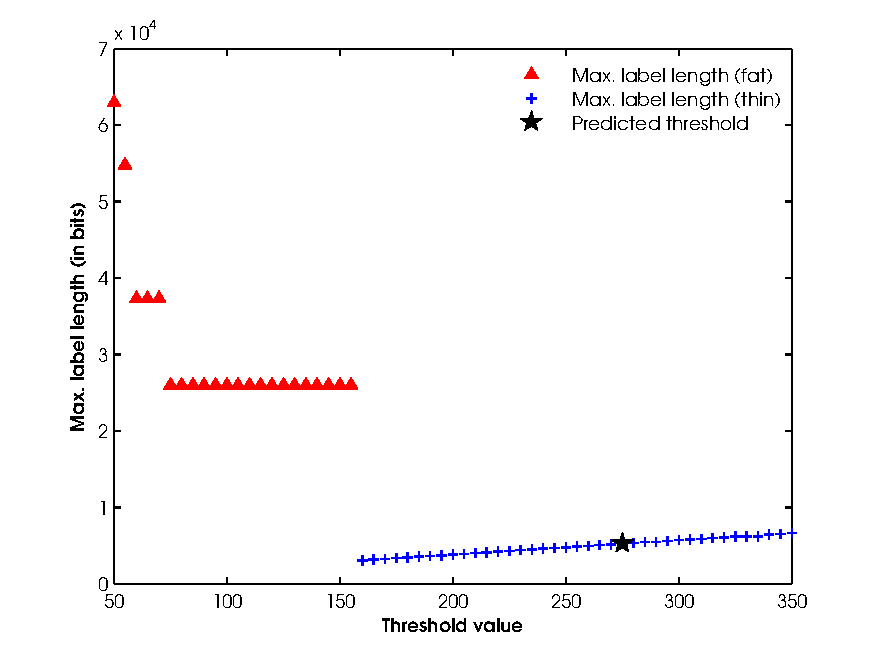
\includegraphics[width=0.4\textwidth]{Figures/barabasi-www.pdf}
}
\subfloat[\small Power law fit]{
    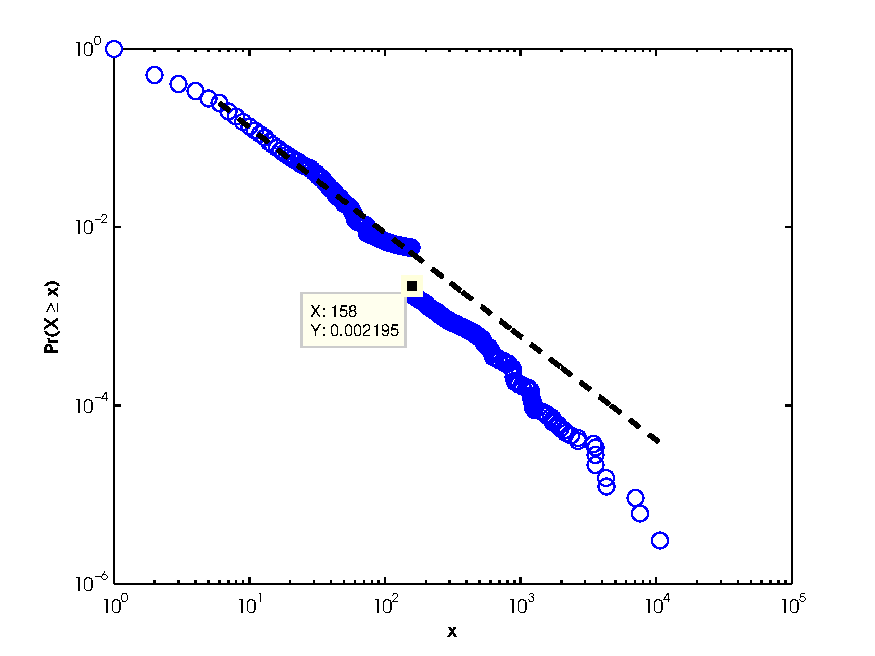
\includegraphics[width=0.4\textwidth]{Figures/barabasi-www-ccdf.pdf}
}%
\quad
\subfloat[\small Fat and thin vertices vs. threshold values]{
    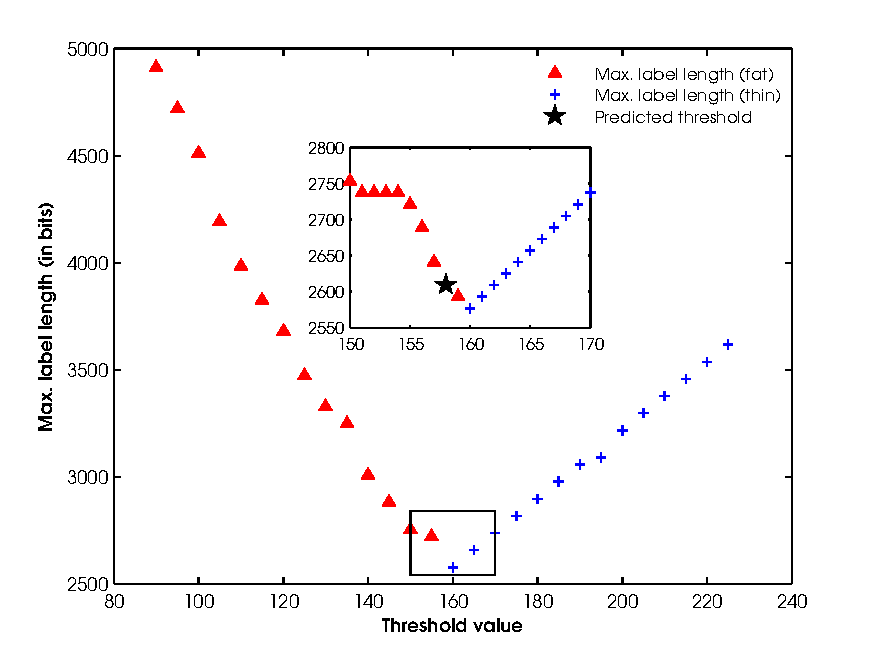
\includegraphics[width=0.4\textwidth]{Figures/enron-mail.pdf}
}
\subfloat[\small Power law fit]{
    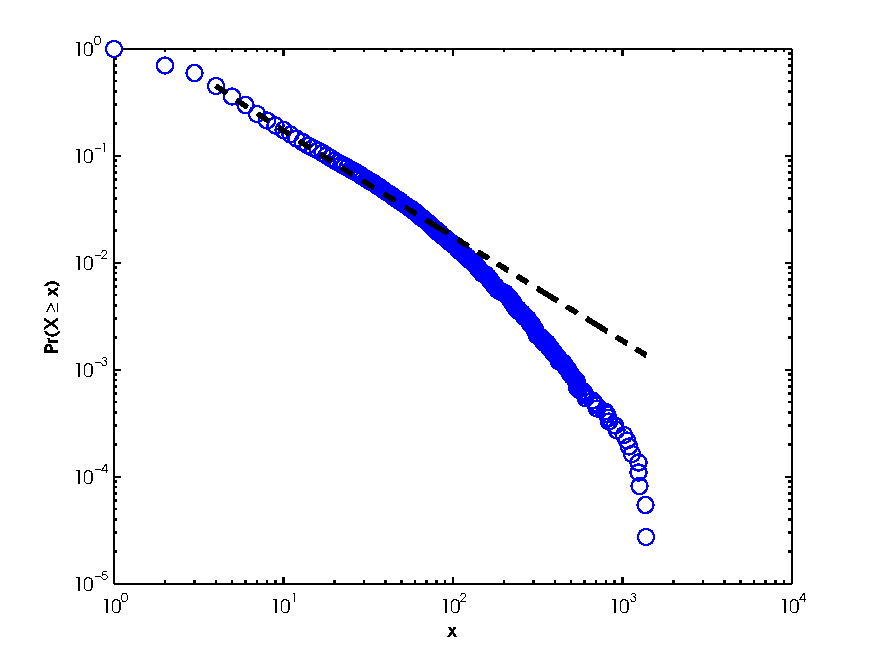
\includegraphics[width=0.4\textwidth]{Figures/enron-mail-ccdf.pdf} 
}%
\quad
\subfloat[\small Fat and thin vertices vs. threshold values]{
    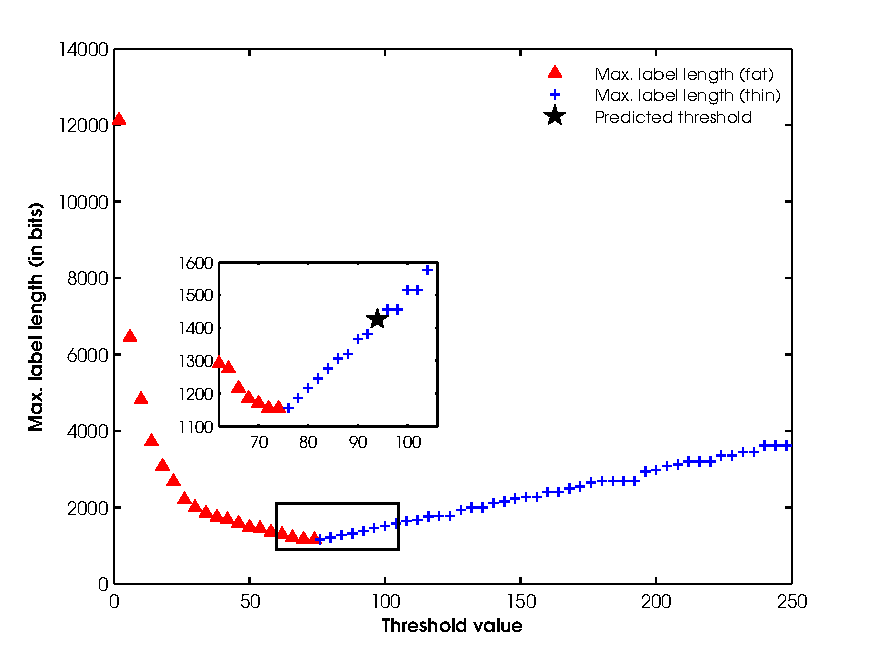
\includegraphics[width=0.4\textwidth]{Figures/internet.pdf}
}
\subfloat[\small Power law fit]{
    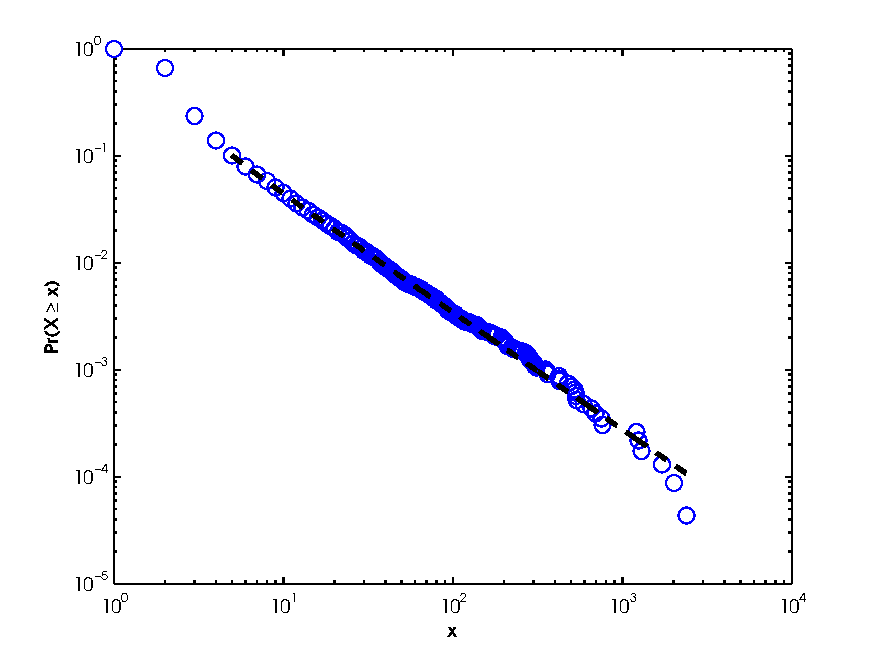
\includegraphics[width=0.4\textwidth]{Figures/internet-ccdf.pdf}
}%
\caption{Left: Fat and thin vertices plotted against increasing threshold values for the \textsc{enron} email communication dataset. The black pentagram is the predicted threshold ($1/\zeta(\alpha)\sqrt[\alpha](n)$) rounded to the nearest integer.  Right: Best-fitting power law ($\alpha = 1.97$)  superimposed on the complementary cumulative distribution function (CCDF) using the framework by \cite{clauset2009power}.}%
\label{fig:synthetic300}%
\end{figure*}


Table~\ref{t:labelsizes}  shows  the maximum label sizes achieved using different labeling schemes on our data sets. ``Predicted'' shows the experimental maximum label size obtained by running our scheme on the graphs, ``Empirical'' is the label size attained by using the empirical threshold.
``Label Diff.'' shows the ratio between the predicted and empirical label sizes, and  ``Threshold Diff.'' shows the ratio between the absolute difference of the threshold values and the maximum degree.
 The remaining columns show non-experimental upper bounds for different label schemes: ``Bound'' is the upper bound guaranteed in Theorem~\ref{prop:labelingMain}, ``$c$-sparse'' is  the labeling scheme for sparse graphs defined in Theorem~\ref{sparse-label}, ``BD'' is the $\lceil \frac{\Delta}{2} \rceil \lceil \log n\rceil$ bounded degree graph  labeling of~\cite{adjiashvili2014labeling}, and AKTZ is the $\lceil n/2\rceil+6$ general graph  labeling of~\cite{alstrup2014adjacency}.
For the dataset groups "Real-Life" and "Synthetic" ``Empirical'' and  ``Bound'' use simple concatenation of labels to represent the fat bit string for "Real-Life" and "Synthetic" , this incurs a $(\log n)/\alpha$ factor on the label size.
The computation of the predicted and empirical bounds for the "Real-Life Large Graphs" datasets was done using the observation that in our original labeling scheme the following holds: Given a  graph $G=(V,E)$, and threshold $t$, with $v_t \in V$ nodes of degree larger than $t$, the label size is $\max{v_t,t \log n}$.

\begin{table*}
\small
\begin{tabular}{ccccccccc}
\hline \multicolumn{9}{c}{Real-Life Graphs}\\\hline
Data set&Predicted &Empirical & Label Diff. & Threshold Diff.   & Upper-Bound     &$c$-sparse &Bounded Degree \cite{adjiashvili2014labeling} &AKTZ \cite{alstrup2014adjacency}\\\hline
\textsc{internet}   &$1,426$    &$1,156$  & $19.0\%$  & $0.8\%$  & $8,181 $  &$4,700$      &$17,925$  &$11,487$\\
\textsc{enron}      &$2,609$    &$2,577$  & $1.3\%$ & $0.2\%$   & $15,835 $ &$9,735$      &$11,056$  &$18,352$\\
\textsc{www}        &$5,245$    &$3,060$  & $41.7\%$  & $1\%$  & $29,225 $ &$28,445$     &$101,840$ &$162,870$ \\
\hline \multicolumn{9}{c}{Real-Life Large Graphs}\\\hline
\textsc{google} & $3,311$ & $2,060$ & $161\%$ & $0.5\%$ & $6,505$ & $24,109$ & $63,320$ & $458,220$\\
\textsc{Youtube}        &$10,596$    &$3,212$  & $329\%$  & $1.3\%$  & $21,7190$ &$25,872$     &$301,917$ &$578,920$ \\
\textsc{WikiTalk}       & $6,972$ & $4,560$ & $152\%$ & $0.1\%$ & $16,664$ & $41,110$ & $1,100,352$ & $1,197,199$\\ 
\textsc{LiveJournal}        &$61,898$    &$7,836$  & $790\%$  & $1.5\%$  & $8,313$ &$56,916$     &$162,976$ &$2,018,275$ \\\hline
\multicolumn{9}{c}{Synthetic Graphs}\\\hline
Data set&Predicted &Empirical & Label Diff. & Threshold Diff.   & Upper-Bound     &$c$-sparse &Bounded Degree \cite{adjiashvili2014labeling} &AKTZ \cite{alstrup2014adjacency}\\\hline
s1M$^{\alpha=2.4}$  &$4,841$    &$4,821$  & $0.4\%$ & $0.002\%$  & $25,012 $ &$30,079$     &$426,820$ &$500,006$\\
s1M$^{\alpha=2.6}$  &$3,361$    &$3,201$   & $4.8\%$ & $0.08\%$  & $15,282 $ &$26,551$     &$121,680$ &$500,006$\\
s1M$^{\alpha=2.8}$  &$2,101$    &$2,061$    & $2\%$ & $0.17\%$  & $10,081 $ &$24,566$     &$16,920$  &$500,006$\\
s300$^{\alpha=2.2}$ &$4,523$    &$4,447$  & $1.7\%$ & $0.05\%$  & $24,878 $ &$18,885$     &$103,607$ &$150,006$\\
s300$^{\alpha=2.4}$ &$2,775$    &$2,680$   & $3.5\%$  & $0.3\%$ & $14,404 $ &$15,420$     &$31,008$  &$150,006$\\
s300$^{\alpha=2.6}$ &$1,958$    &$1,920$  & $3.1\%$ & $0.35\%$   & $9,151 $  &$13,792$     &$13,395$  &$150,006$\\
s300$^{\alpha=2.8}$ &$1,350$    &$1,312$  & $2.8\%$ & $0.1\%$   & $6,244 $  &$12,849$     &$17,499$  &$150,006$\\\hline
\end{tabular}
\caption{Label size in bits of labeling schemes. The two leftmost columns are experimental results; Label Diff. and  Threshold Diff. column  report findings related to  performance indicator ii, and the remaining are upper bounds on label sizes computed from the characteristics of the data sets.}
\label{t:labelsizes}
\end{table*}

Our findings are as follows.
For Performance Indicator (i), both our experimental results and theoretical upper bounds for our labeling scheme are several orders of magnitudes lower than for labeling schemes aimed at more general classes of graphs, as expected. Of the more general classes of graphs, it is most interesting to compare the upper bound of bounded degree graphs---the most restrictive class of graphs that both contains the class of power-law graphs and has an efficient labeling scheme described in the literature~\cite{adjiashvili2014labeling}. As seen in Table \ref{t:labelsizes}, the upper bound on our labeling schemes for both power-law graphs and sparse graphs have better upper bounds on label sizes, but only marginally so for data sets with low maximum degree and low values of the power-law parameter $\alpha$, e.g. \textsc{Enron} ($\alpha = 1.97$). 
The actual label sizes obtained in the experiments (the two leftmost columns of Table \ref{t:labelsizes}) are substantially lower than the upper bounds, that is, the labeling scheme performs much better in practice than suggested by theory (down to less than a kilobyte per vertex for all data sets). 
This phenomenon may be due to the degree distribution of the graphs of the data sets having only minor deviation from a power-law for small vertex degrees; our upper bounds on the label size are derived by using the very rich family $\PLB$ that allows very large deviation from a power-law for degrees between $1$ and $\sqrt[\alpha]{n/\log n} - 1$.

 For Performance Indicator (ii), our labeling scheme obtains maximum label size at most 3.5\% larger than what would have been obtained by using the empirical threshold for all synthetic data sets.
This is expected---the synthetic data sets are graphs generated specifically to have power-law distributed degree distribution. 
For the real-world data sets, the labeling scheme obtains maximum label much larger than the empirical threshold; this larger deviation is likely due to degree distributions of the data sets being close to, but not quite,
power-law distributions due to natural phenomena or noise. E.g., for the \textsc{enron} data set there is sudden drop in frequency between nodes of degree $< 158$ and $\geq 158$. Despite the large difference in label size, we note that the threshold difference never exceeds $1.5\%$. This implies that using the theoretical threshold to speed up the labeling is a valid step even for graphs that are not perfectly power-law.


Finally, note that our labeling scheme supports adjacency for \emph{directed} graphs by using one more bit per edge in each label to store the edge orientation.
\section{Conclusion and Future Work}
We have devised adjacency and distance labeling schemes for sparse graphs and graphs whose degree distribution approximately follows a power-law distribution.
 We have proven lower bounds for the class of power-law graphs showing that our strategy for adjacency labeling scheme is  almost  optimal. 
 Furthermore, we have shown experimentally that the labeling scheme for power-law graphs obtain
results in practice requiring little  space, and that the theoretical threshold we use in our strategy is reasonably close to the optimum threshold.

\subsection{Future work}
We propose the following directions:
\begin{itemize}
\item{Our labeling schemes are designed for static networks, and while it seems not difficult to extend our idea to dynamic networks, an analysis is required to account for the communication and number of re-labels such an extension will incur.}
\item{Labeling schemes for power law graphs can likely be devised for the realistic case where the scheme only has incomplete knowledge of the graph, for example when the expected frequency of vertices of each degree is known, but not the exact frequency of each vertex.}
%As our labeling scheme can be extended to handle directed graphs by using a single bit more per label, 
\item{One way to view labeling schemes as a hole is the extreme scenario where our data structure is disseminated across $n$ machines.
This may lead to a better understanding of  overheads observed in other  distributed graph storage technics.}
%\item{The entropy of both the Chung-Liu and the BA model was recently determined to be similar. It is thus quite surprising that the label size difference is as large as we have proved. It is thus conjectured that the number of nodes of large label size is very small for this family.}
\item{Closing the  gap of the multiplicative logarithmic factor may be  of interest to the theory community. A much more interesting gap exists for distance labeling schemes.
As we have seen, there is a large gap between labeling schemes for short distance and adjacency for power-law (and sparse) graphs.
This gap effectively deemed the distance labels uninteresting for practical applications.}
\item{Finally, while power-law distributions may model the degree distribution of real-world networks, other distributions
may fit better (see, e.g., \cite{clauset2009power}); it is interesting to see whether refinements of our labeling scheme that utilize knowledge about such distributions would result in superior labeling schemes for real-world data.}
\end{itemize}

